\section{Broker}


Das Broker Architektur Pattern kann zur Strukturierung von verteilten Systemen mit abgekoppelten Komponenten benutzt werden, welche durch entfernte (remote) Service-Aufrufe interagieren.

\subsection*{Example}


Nehmen wir an wir entwickeln ein City Information System (CIS) in einem WAN laufen soll. Einige Computer des Netzwerkes stellen einen oder mehrere Services zur Verfügung, welche Informationen über Events, Restaurants, Hotels, Historische Denkmäler oder den öffentlichen Verkehr verwalten. Touristen können diese Informationen mit Terminals über einen World Wide Web (WWW) Browser abrufen. Diese Front-End Software ruft die online Informationen von entsprecheden Server ab und zeigt sie auf dem Bildschirm an. Die Daten werden üer das Netzwerk verteilt und nicht durch die Terminals verwaltet.

Da das System laufend Änderungen unterworfen ist und stetig wächst sollen die individuellen Services voneinander entkoppelt sein. Zudem sollen die Terminals zugriff auf die Services haben ohne ihren Ort zu kennen. Dies erlaubt es die Services zu bewegen, replizieren oder zu migrieren. Eine Lösung ist es ein eigenständiges Netzwerk, welches die Terminals mit den Servern verbinden, zu installieren (Intranet System). Dieser Ansatz hat jedoch einige Nachteile: nicht jeder Zulieferer von Informationen will sich mit einem geschlossenen Intranet verbinden, zudem sollen die Services weltweit zur Verfügung stehen. Das Internet ist dadurch besser geeignet das CIS system zu implementieren.

\subsection*{Context}


Deine Umgebung ist ein verteiltes und möglicherweise heterogenes System mit unabhängigen, zusammenarbeitenden Komponenten.

\subsection*{Problem}


Ein System als Menge von losen und kommunizierenden Komponenten bauen, anstelle einer monolitischen Applikation, bringt grössere Flexibilität, Wartarbkeit und Anpassbarkeit. Durch das Unterteilen der Funktionalität in unabhängige Komponenten wird die Verteilbarkeit und Skalierbarkeit des Systems unterstützt.

Allerdings ist zur Kommunikation der Komponenten eine Form von Interprozess-Kommunikation nötig. Falls die Komponenten die Kommunikation selbst handhaben, hat das resultierende System mit verschiedenen Abhängigkeiten und Einschränkungen zu kämpfen.

Diese um Komponenten hinzuzufügen, zu entfernen, auszuwechseln, zu aktiveiren und zu orten werden ebenfalls benötigt.

\subsection*{Forces}


\begin{itemize}
	\item Komponenten sollen auf Dienste (Services) von anderen Komponenten zugriffen können durch ein entfernte, orts-transparente Dienstaufrufe (remote, location-transparent service invocationen)
	\item Es ist nögit Komponenten zur Laufzeit auszuwechseln, hinzuzufügen oder zu entfernen.
	\item Die Architektur soll system- und implementationsspezifische Details vor den Benutzern der Komponenten und Dienste verbergen.
\end{itemize}

\subsection*{Solution}


Führe eine Broker-Komponente (Vermittler) ein um eine bessere Entkopplung von Clients und Server zu erreichenn. Server registieren sich beim Broker und stellen ihre Dienste (Services) über eine Methoden-Schnittstelle (method interface) den Clients zur Verfügung. Clients greiffen auf die Funktionalität zu indem sie Anfragen an den Broker senden. Die Aufgabe des Brokers beinhaltet den entsprechenden Server zu finden, die Anfrage an den Server weiterzuleiten und die Resultate und Exception zurück an den Client zu reichen.

Durch das Broker-Pattern kann eine Anwendung auf verteilte Dienste zugreifen indem sie einfach Nachrichten (message calls) zum entsprechenden Objekt schickt, anstatt sich selbst um die low-level Interprozess zu kümmern.

Das Broker-Pattern reduziert die Komplexität beim Entwickeln von verteilten Anwendungen, da es die Verteilung für den Entwickler transparent macht. Dies erreicht es adurch, das ein Objektmodell eingeführt wird in welchem die verteilten Dienste durch Objekte gekapselt werden.

\subsection*{Structure}


\begin{figure}[H]
	\centering
	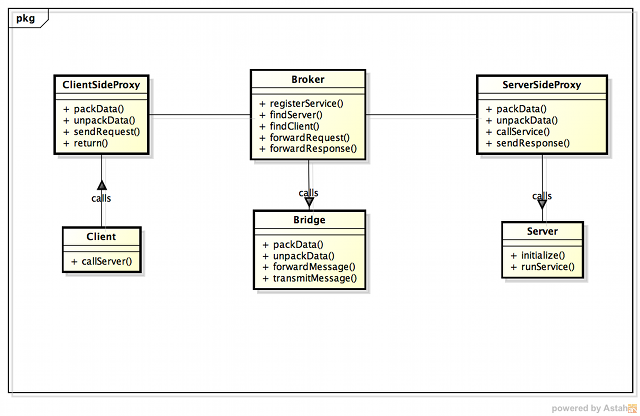
\includegraphics[width=0.7\textwidth]{content/posa1/images/broker-classes.png}
	\caption{Broker}
\end{figure}


Das Broker-Architektur-Pattern besteht aus sechs Arten von teilnehmenden Komponenten: Clients, Servers, Brokers, Bridges, Client-Side-Proxies und Server-Side-Proxies.

Ein Server implementiert objekte welche ihre Funktionalität durch einheitliche Schnittstellen (Interfaces) zur Verfügung stellen. Diese Schnittstellen werden entweder durch eine Interface Definition Language (IDL) oder durch einen binären Standard verfügar gemacht.

Clients sind Anwendungen welche auf mindestens einen Server zugreifen. Um einen entfernten Dienst (remote service) zu nutzen, schickt ein Client eine Anfrage (Request) an den Broker.

Ein Broker ist ein Bote welcher verantwortlich ist die Anfragen von Clients an Servers, wie auch die Antworten und Exceptions vom Servers zurück an Clients zu übertragen. Abhängig von den Anforderungen des Gesammtsystems können weitere Dienste, wie Namensdienste (name services) oder Marshalling, in den Broker integriert werden.

Client-Side-Proxies stellen den Layer zwischen Clients und Broker dar. Dieser zusätzliche Layer bietet Transparenz, so dass ein entferntes Objekt (remote object) wie ein lokales Objekt erscheint. Zudem werden Implementationsdertails vor den Clients verborgen, wie zum Beispiel die Interprozesskommunikation, Speicherverwaltung und Marshalling (Umwandeln von Datenformaten in andere Darstellungen).

Server-Side-Proxies funtionieren wie Client-Side-Proxies. Der Unterschied ist dass sie Verwantwortlich sind, Anfragen entgegenzunehmen, eingehende Nachrichten zu entspacken, das Unmarshalling durchzuführen und den nötigen Dienst aufzurufen.

Bridges sind optionale Komponenten welche Implementationsdetails verbergen wenn zwei Brokers zusammenarbeiten.

Es gibt zwei verschiedene Arten von Broker-Systemen: solche welche eine direkte und solche welche eine indirekte Kommunikation nutzen. Um eine bessere Performance zu erreichen, bauen manche Broker-Systeme nur die initiale Kommunikationsverbindung zwischen Client und Server auf, während der Rest der Kommnunikation direkt zwischen den beiden Komponenten stattfindet. In dieser Pattern Beschreibung wird auf die indirekte Broker Variante eingegangen, bei der jegliche Kommunkations über den Broker stattfindet.

\subsection*{Dynamics}

\subsubsection*{Szenario 1: Ein Server registriert sich bei der lokalen Broker-Komponente}

\begin{figure}[H]
	\centering
	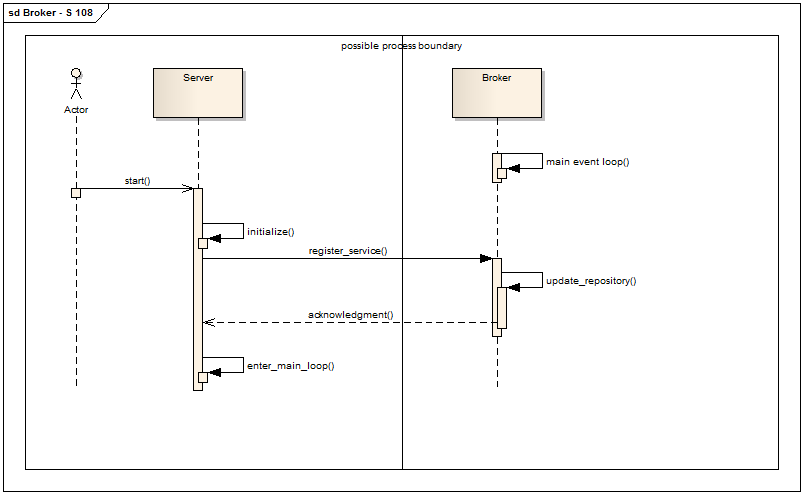
\includegraphics[width=0.7\textwidth]{content/posa1/images/broker-scen1.png}
	\caption{Broker Szenario 1}
\end{figure}

\begin{enumerate}
	\item Der Broker startet die Initialisierung und wartet in einem Event-Loop auf eingehende Nachrichten.
	\item Der Benutzer startet eine Server-Anwendung, welche sich erst initialsiert und sich daraufhin beim Broker registriert.
	\item Der Broker erhält die eingehenden Registrierungsanfrage des Servers und speichert diese in einer Art Repository. Das Repository wird benötigt um die Server zu lokaliseren und zu aktivieren.
	\item Nachdem der Server die Registrierungsbestägigung des Brokers erhalten hat warten der Server in einem eigenen Loop auf eintreffende Client-Anfragen.
\end{enumerate}


\subsubsection*{Szenario 2: Ein Client sendet eine Anfrage an einen lokalen Server}

\begin{figure}[H]
	\centering
	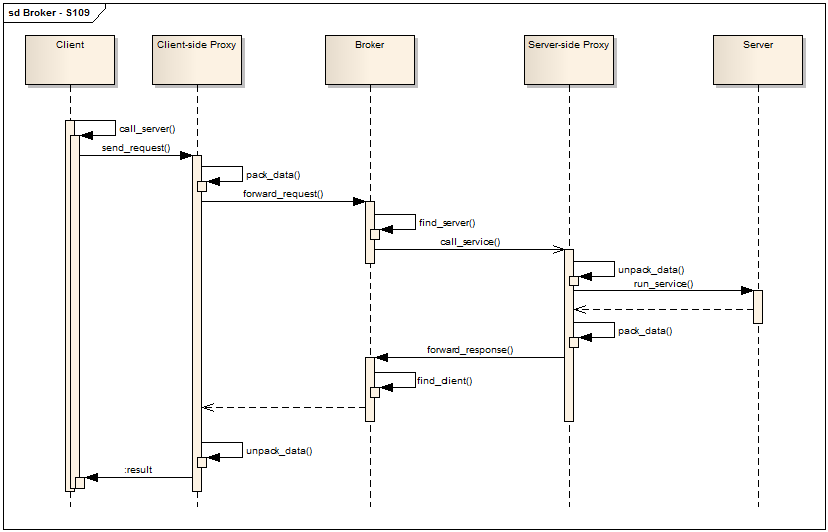
\includegraphics[width=0.7\textwidth]{content/posa1/images/broker-scen2.png}
	\caption{Broker Szenario 2}
\end{figure}

\begin{enumerate}
	\item Die Client-Anwendung startet und ruft während der Ausführung eine Methode eines Remote-Server-Objekts auf.
	\item Der Client-Side-Proxy verpackt alle nötigen Informationen in eine Nachricht und sendet sie an den lokalen Broker.
	\item Der Broker sucht den passenden Server aus seinem Repository heraus und leitet die Nachricht an den entsprechenden Server-Side-Proxy weiter.
	\item Der Server-Side-Proxy entpackt die Informationen aus der Nachricht und ruft den entsprechenden Dienst auf.
	\item Nachdem die Ausführung komplett ist, gibt der Server das Resultat an den Server-Side-Proxy zurück, welcher die Informationen in eine Nachricht verpackt und sie an den Broker weitergibt.
	\item Der Broker leitet die Nachricht an den entsprechenden Client-Side-Proxy weiter.
	\item Der Client-Side-Proxy erhält die Antwort, entpackt das Resultat und gibt es an die Client-Anwendung zurück.
\end{enumerate}

\subsubsection*{Szenario 3: Interaktion von mehreren Brokern mit Hilfe von Bridge-Komponenten}

\begin{figure}[H]
	\centering
	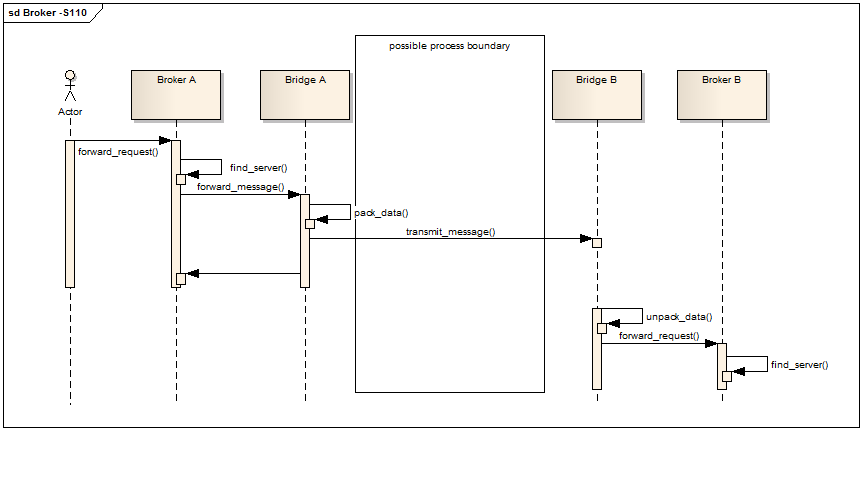
\includegraphics[width=0.7\textwidth]{content/posa1/images/broker-scen3.png}
	\caption{Broker Szenario 3}
\end{figure}

\begin{enumerate}
	\item Broker A empfängt eine Anfrage und sieht in seinem Repository nach, welche Server dafür zuständig ist. Da sich der Server in einem anderen Netzwerkknoten (network node) befindet, leitet der Broker die Nachricht an einen entfernten Broker (remote Broker) weiter.
	\item Die Nachricht wird von Broker A zur Bridge A weitergeleitet. Diese konvertiert die Nachricht in ein Format, welches beide Bridges verstehen. Bridge A sendet die Nachricht daraufhin an Bridge B.
	\item Bridge B bildet die eingehende Anfrage auf ein für Broker B spezifisches Format ab.
	\item Broker B führt die notwendigen Schritte aus wenn eine Anfrage eintrifft.
\end{enumerate}

\subsection*{Implementation}

\begin{enumerate}
	\item Definiere ein Objekt-Modell oder benutze ein bestehendes Modell.
	\item Entscheide welche Art der Komponenten-Komunikation (component-interoperability) das System bereitstellen soll.
	\item Spezifiziere die APIs der Broker-Komponente für die Zusammenarbeit von Clients und Servers.
	\item Benutze Proxy-Objekte um die Implementationsdetails vor Clients und Servers zu verbergen.
	\item Entwirf die Broker-Komponente parallel zu Schritt 3 und 4.
	\item Entwickle IDL-Compiler. Falls die Interoperabilität durch eine Interface Definiton Language (IDL) geschieht, so muss man einen IDL Compiler für jede unterstützte Programmiersprache zur Verfügung stehen.
\end{enumerate}


\subsubsection*{Variants}
\begin{itemize}
	\item Direct Communication Broker System. Nachrichten werden nur über den Broker ausgetauscht.
	\item Message Passing Broker System. Server benutzen den Typ einer Nachricht um zu entscheiden was zu tun ist.
	\item Trader Sytem. Eine Anfrage eines Clients wird zu genau einem eindeutigen Server weitergereicht.
	\item Adapter Broker System. Ein zusätzlicher Adapter verbirgt die Schnittstelle der Broker-Komponente für zusätzliche Flexiblität.
	\item Callback Broker System. Statt einem aktiven Kommunikationsmodell kann auch ein reaktives Modell benutzt werden. Das reaktive Modell ist ereignissgesteuert und unterscheidet nicht zwischen Clients und Servers.
\end{itemize}

\subsection*{Known Uses}


\begin{itemize}
	\item CORBA
	\item IBM SOM/DSOM
	\item Microsoft OLE 2.x
	\item World Wide Web
	\item ATM-P. Telekommunikations Switch-System von Siemens.
\end{itemize}

\subsection*{Consequences}


\subsubsection*{Benefits}


\begin{itemize}
	\item Testing und Debugging. Die einzelnen Komponente lassen sich gut testen, das gesammte Broker-System mit den vielen Komponenten als gesammtes ist allerdings sehr mühsam zu testen.
	\item Orts-Transparenz. Clients müssen den genauen Ort der Server nicht kennen.
	\item Änderbarkeit und Erwartbarkeit von Komponenten.
	\item Portabilität des Broker-Systems.
	\item Interoperablität zwischen verschiedenen Broker-Sytemen
	\item Wiederverwendbarkeit
\end{itemize}

\subsubsection*{Liabilities}


\begin{itemize}
	\item Testing und Debugging. Die einzelnen Komponente lassen sich gut testen, das gesammte Broker-System mit den vielen Komponenten als gesammtes ist allerdings sehr mühsam zu testen.
	\item Beschränkte Effizienz.
	\item Geringere Fehlertoleranz
\end{itemize}



\subsection*{See also}

\begin{itemize}
	\item Forwarder-Receiver Pattern für die interprozess Kommunikation
	\item Proxy-Pattern
	\item Client-Dispatcher-Server Pattern
	\item Mediator Design Pattern
\end{itemize}